%
% Copyright 2021 Joel Feldman, Andrew Rechnitzer and Elyse Yeager.
% This work is licensed under a Creative Commons Attribution-NonCommercial-ShareAlike 4.0 International License.
% https://creativecommons.org/licenses/by-nc-sa/4.0/
%
\graphicspath{{figures/odeNumerical/}}
%\renewcommand{\theequation}{\thechapter.\arabic{equation}}
%\renewcommand{\thetheorem}{\thechapter.\arabic{theorem}}
%\renewcommand{\thebc}{\thechapter.\arabic{theorem}}
%\renewcommand{\theeg}{\thechapter.\arabic{theorem}}

\chapter{Numerical Solution of ODE's}\label{app ODE numerical}
In Section~\ref{sec sep de} we solved a number of inital value problems of the 
form
\begin{align*}
y'(t)&=f\big(t,y(t)\big) \\
y(t_0)&=y_0
\end{align*}
Here $f(t,y)$ is a given function, $t_0$ is a given initial time and
$y_0$ is a given initial value for $y$. The unknown in the problem is the
function $y(t)$. There are a number of other techniques for analytically 
solving some problems of this type. However it is often simply not 
possible to find an explicit solution. This appendix introduces some 
simple algorithms for generating approximate numerical solutions to 
such problems. 

\section{Simple ODE Solvers --- Derivation}
The first order of business is to derive three simple algorithms for
generating approximate numerical solutions to the initial value problem
\begin{align*}
y'(t)&=f\big(t,y(t)\big) \\
y(t_0)&=y_0
\end{align*}
The first is called Euler's method because it was developed by (surprise!) 
Euler\footnote{Leonhard Euler (1707--1783) was a  Swiss mathematician and physicist who spent most of his adult life in Saint Petersberg and Berlin. He gave the name $\pi$ to the ratio of a circle's circumference to its diameter. He also developed the constant $e$.}.
%%%%%%%%%%%%% 
\subsection{Euler's Method}\label{ap_euler}
%%%%%%%%%%%%%
Our goal is to approximate (numerically) the unknown function 
\begin{align*}
y(t) &= y(t_0) + \int_{t_0}^t y'(\tau)\,\dee{\tau} \\
     &= y(t_0) + \int_{t_0}^t f\big(\tau,y(\tau)\big)\,\dee{\tau}
\end{align*} 
for $t\ge t_0$.  We are told explicitly the value of $y(t_0)$, namely $y_0$.
So we know $f\big(\tau,y(\tau)\big)\big|_{\tau=t_0}=f\big(t_0,y_0\big)$.
But we do not know the integrand $f\big(\tau,y(\tau)\big)$ for $\tau>t_0$.
On the other hand, if $\tau$ is close $t_0$, then $f\big(\tau,y(\tau)\big)$ will remain close\footnote{This will be the case as long as $f(t,y)$ is continuous.} 
to $f\big(t_0,y_0\big)$. So pick a small number $h$ and define 
\begin{align*}
t_1&=t_0+h \\
y_1&=y(t_0) + \int_{t_0}^{t_1} f(t_0,y_0)\,\dee{\tau}
   =y_0+f\big(t_0,y_0\big)(t_1-t_0) \\
  &=y_0+f\big(t_0,y_0\big)h
\end{align*} 
By the above argument 
\begin{equation*}
y(t_1)\approx y_1 
\end{equation*}


%Our goal is to approximate (numerically) the unknown function $y(t)$ for
%$t\ge t_0$. We are told explicitly the value of $y(t_0)$,
%namely $y_0$. Thanks to the given differential equation, we can also use $y_0$
%to find the exact instantaneous rate of change of $y$ at time $t_0$.
%\begin{equation*}
%y'(t_0)=f\big(t_0,y(t_0)\big)=f\big(t_0,y_0\big)
%\end{equation*}
%If the rate of change of $y(t)$ were to remain constant at 
%$f\big(t_0,y_0\big)$ for all time, then $y(t)$ would be exactly $y_0+f\big(t_0,y_0\big)(t-t_0)$.
%However, the rate of change of $y(t)$ does not remain $f\big(t_0,y_0\big)$ for
%all time, but it is not unreasonable to expect that when  $t$ is close 
%to $t_0$, the rate of change stays close to $f\big(t_0,y_0\big)$. 
%If this is the case, then the value of $y(t)$ will remain close to
%$y_0+f\big(t_0,y_0\big)(t-t_0)$ for $t$ close to $t_0$. So pick a small
%number $h$ and define 
%\begin{align*}
%t_1&=t_0+h \\
%y_1&=y_0+f\big(t_0,y_0\big)(t_1-t_0)=y_0+f\big(t_0,y_0\big)h
%\end{align*} 
%That is, we approximate the solution by pretending that $f$ does not change on the very small interval $t_0\le t\le t_0+h$.
%By the above argument 
%\begin{equation*}
%y(t_1)\approx y_1 
%\end{equation*}

\begin{efig}
\begin{center}
%    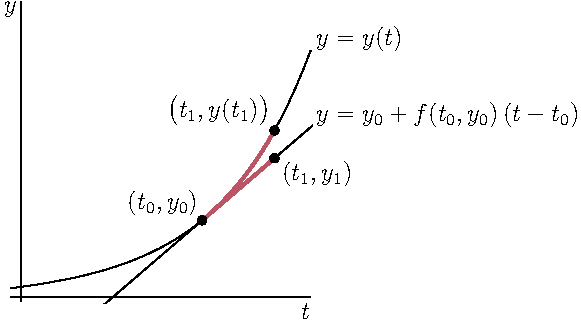
\includegraphics[scale=1.3]{eulerIntro.pdf}
    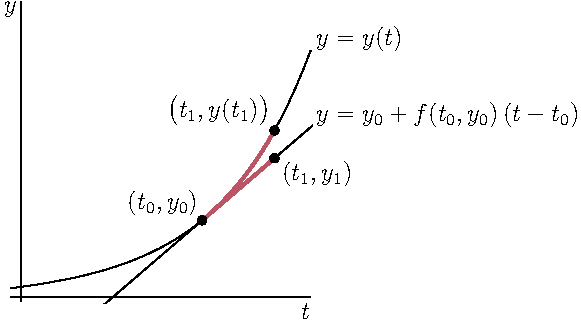
\includegraphics{eulerIntro.pdf}
\end{center}
\end{efig}

Now we start over from the new point $(t_1,y_1)$. We now know an approximate value for $y$ at time $t_1$.
If $y(t_1)$ were exactly $y_1$, then the instantaneous rate of change of 
$y$ at time $t_1$, namely $y'(t_1)=f\big(t_1,y(t_1)\big)$, would be exactly 
$f(t_1,y_1)$ and  $f\big(t,y(t)\big)$ would remain close to $f(t_1,y_1)$
for $t$ close to $t_1$. Defining
\begin{align*}
t_2&=t_1+h=t_0+2h \\
y_2&=y_1 + \int_{t_1}^{t_2} f(t_1,y_1)\,\dee{t}
   =y_1+f\big(t_1,y_1\big)(t_2-t_1) \\
  &=y_1+f\big(t_1,y_1\big)h
\end{align*}
we have 
\begin{equation*}
y(t_2)\approx y_2 
\end{equation*}


%Now we start over from the new point $(t_1,y_1)$. We now know the approximate value of $y$ at time $t_1$.
%If $y(t_1)$ were exactly $y_1$, then the instantaneous rate of change of 
%$y$ at time $t_1$ would be exactly $f(t_1,y_1)$. If this rate of change
%were to persist for all future time, $y(t)$ would be exactly
%$\ y_1+f\big(t_1,y_1\big)(t-t_1)\ $. As $y(t_1)$ is only approximately
%$y_1$ and as the rate of change of $y(t)$ varies with $t$, the rate 
%of change of $y(t)$ is only approximately $f(t_1,y_1)$ and only for 
%$t$ near $t_1$. So we approximate $y(t)$ by $\ y_1+f\big(t_1,y_1\big)(t-t_1)\ $
%for $t$ bigger than, but close to, $t_1$. Defining
%\begin{align*}
%t_2&=t_1+h=t_0+2h \\
%y_2&=y_1+f\big(t_1,y_1\big)(t_2-t_1)=y_1+f\big(t_1,y_1\big)h
%\end{align*}
%we have 
%$$
%y(t_2)\approx y_2 
%$$

We just repeat this argument ad infinitum. Define, for $n=0,1,2,3,\cdots$
\begin{equation*}
t_n=t_0+nh
\end{equation*}
Suppose that, for some value of $n$, we have already computed an approximate
value $y_n$ for $y(t_n)$. Then the rate of change of $y(t)$
for $t$ close to $t_n$ is 
$f\big(t,y(t)\big)\approx f\big(t_n,y(t_n)\big)\approx f\big(t_n,y_n\big)$
and
\begin{impeqn}[Euler's Method]\label{Eul}
\begin{equation*}
y(t_{n+1})\approx y_{n+1}=y_n+f\big(t_n,y_n\big)h
\end{equation*}
\end{impeqn}\noindent
%We just repeat this argument ad infinitum. Define, for $n=0,1,2,3,\cdots$
%\begin{equation*}
%t_n=t_0+nh
%\end{equation*}
%Suppose that, for some value of $n$, we have already computed an approximate
%value $y_n$ for $y(t_n)$. Then the rate of change of $y(t)$
%for $t$ close to $t_n$ is 
%$f\big(t,y(t)\big)\approx f\big(t_n,y(t_n)\big)\approx f\big(t_n,y_n\big)$
%and, again for $t$ close to $t_n$, $y(t)\approx y_n+f\big(t_n,y_n\big)(t-t_n)$.
%Hence
%\begin{impeqn}[Euler's Method]\label{Eul}
%\begin{equation*}
%y(t_{n+1})\approx y_{n+1}=y_n+f\big(t_n,y_n\big)h
%\end{equation*}
%\end{impeqn}
This algorithm is called \emph{Euler's Method}. The parameter $h$ is called
the \emph{step size}. 

Here is a table applying a few steps of Euler's method
to the initial value problem 
\begin{align*}
y'&=-2t+y \\
y(0) & = 3
\end{align*}
with step size $h=0.1$. For this initial value problem
\begin{align*}
f(t,y)&=-2t+y \\
t_0&=0 \\
y_0&=3
\end{align*}
Of course this initial value problem has been chosen for illustrative purposes
only. The exact solution is\footnote{Even if you haven't learned how to solve initial value problems like this one, you can check that $y(t)=2+2t+e^t$ obeys both $y'(t)=-2t+y(t)$ and $y(0)=3$.} $y(t)=2+2t+e^t$.

\begin{center}
\def\arraystretch{1.25}%
\begin{tabular}{ !{\vrule width 1.5pt} c !{\vrule width 1pt} c | c | c | c !{\vrule width 1.5pt}}
\noalign{\hrule height 1.5pt}
$n$ & $t_n$ & $y_n$ & $f(t_n,y_n)=-2t_n+y_n$ & $y_{n+1}=y_n+f(t_n,y_n)*h$ \\
\noalign{\hrule height 1.5pt}
  0 & 0.0 & 3.000 & -2*0.0+3.000=3.000 & 3.000+3.000*0.1=3.300  \\
\hline
  1 & 0.1 & 3.300 & -2*0.1+3.300=3.100 & 3.300+3.100*0.1=3.610  \\
\hline
  2 & 0.2 & 3.610 & -2*  0.2+3.610=3.210 & 3.610+3.210*0.1=3.931 \\
\hline
  3 & 0.3 & 3.931 & -2*  0.3+3.931=3.331 & 3.931+3.331*0.1=4.264 \\
\hline
  4 & 0.4 & 4.264 & -2*  0.4+4.264=3.464 & 4.264+3.464*0.1=4.611 \\
\hline
  5 & 0.5 & 4.611 &  &   \\
\noalign{\hrule height 1.5pt}
\end{tabular}
\def\arraystretch{1.0}%
\end{center}
The exact solution at $t=0.5$ is $4.6487$, to four decimal places. 
We expect that Euler's method will become more accurate as
the step size becomes smaller. But, of course, the
amount of effort goes up as well. If we recompute using $h=0.01$, we get
(after much more work) $4.6446$.

%%%%%%%%%%%%%%%%%%%
\subsection{The Improved Euler's Method}\label{ap_imp_euler}
%%%%%%%%%%%%%%%%%%%
Euler's method is one algorithm which generates approximate solutions to
the initial value problem
\begin{align*}
y'(t)&=f\big(t,y(t)\big) \\
y(t_0)&=y_0
\end{align*}
In applications, $f(t,y)$ is a given function and $t_0$ and $y_0$ are given
numbers. The function $y(t)$ is unknown. Denote by $\varphi(t)$ the exact
solution\footnote{Under reasonable hypotheses on $f$, there is exactly one such solution. The interested reader should search engine their way to the Picard-Lindel\"of theorem.} for this initial value problem. In other words $\varphi(t)$ is
the function that obeys
\begin{align*}
\varphi'(t)&=f\big(t,\varphi(t)\big) \\
\varphi(t_0)&=y_0
\end{align*}
exactly.

Fix a step size $h$ and define $t_n=t_0+nh$. By turning the problem into one 
of approximating integrals, we now derive another algorithm
that generates approximate values for $\varphi$ at the sequence of equally
spaced time values $t_0,\ t_1,\ t_2,\ \cdots$. We shall denote the approximate
values $y_n$ with
\begin{equation*}
y_n\approx\varphi(t_n)
\end{equation*}
By the fundamental theorem of calculus and the differential equation, the 
exact solution obeys
\begin{align*}
\varphi(t_{n+1})&=\varphi(t_n)+\int_{t_n}^{t_{n+1}}\varphi'(t)\ \dee{t} \\
&=\varphi(t_n)+\int_{t_n}^{t_{n+1}}f\big(t,\varphi(t)\big)\ \dee{t}
\end{align*}
Fix any $n$ and suppose that we have already found $y_0,\ y_1,\ \cdots,\ y_n$.
Our algorithm for computing $y_{n+1}$ will be of the form
\begin{equation*}
y_{n+1}=y_n+\text{\ approximate\ value\ of \ }
\int_{t_n}^{t_{n+1}}f\big(t,\varphi(t)\big)\ \dee{t}
\end{equation*}

In Euler's method, we approximated $f\big(t,\varphi(t)\big)$ 
for $t_n\le t\le t_{n+1}$ by
%In fact we can write Euler's method in precisely this form. In Euler's method,
%we approximate $f\big(t,\varphi(t)\big)$ for $t_n\le t\le t_{n+1}$ by
the constant $f\big(t_n,y_n\big)$. Thus
\begin{equation*}
\text{Euler's approximate value for\ }
\int_{t_n}^{t_{n+1}}f\big(t,\varphi(t)\big)\ \dee{t}
\text{ is }\int_{t_n}^{t_{n+1}}f\big(t_n,y_n\big)\ \dee{t}
%=f\big(t_n,y_n\big)[t_{n+1}-t_n]
=f\big(t_n,y_n\big)h
\end{equation*}
So Euler's method approximates the area of the complicated region
$\ 0\le y\le  f\big(t,\varphi(t)\big)$, $t_n\le t\le t_{n+1}\ $
(represented by the shaded region under the parabola in the left half
of the figure below) by the area of the rectangle 
$\ 0\le y\le  f\big(t_n,y_n\big),\ t_n\le t\le t_{n+1}\ $
(the shaded rectangle in the right half
of the figure below).

\begin{efig}
\begin{center}
%    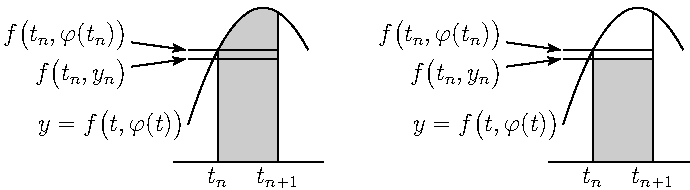
\includegraphics[scale=1.3]{euler.pdf}
    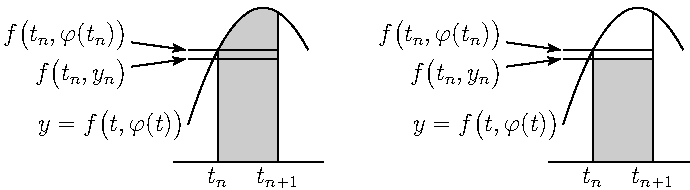
\includegraphics{euler.pdf}
\end{center}
\end{efig}

Our second algorithm, the improved Euler's method, gets a better approximation 
by using the trapezoidal rule. That is, we approximate the integral
by the area of the trapezoid on the right below, rather than the rectangle
on the right above.
\vadjust{
\begin{efig}
\begin{center}
%    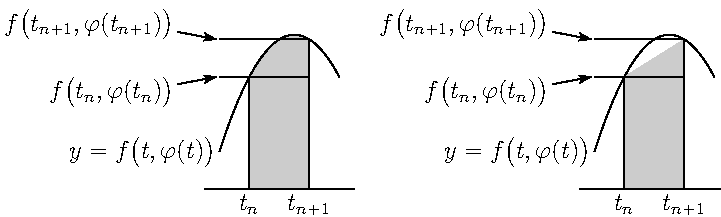
\includegraphics[scale=1.3]{impeuler.pdf}
    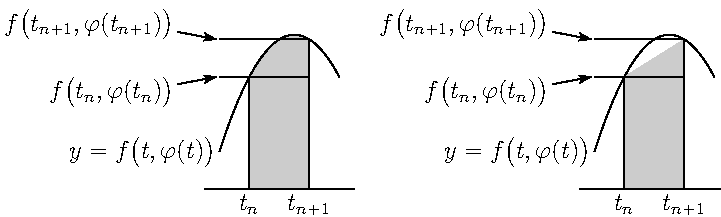
\includegraphics{impeuler.pdf}
\end{center}
\end{efig}
}%%%%%%%
The exact area of this trapezoid is the length $h$ of the base multiplied
by the average of the heights of the two sides, which is $\frac{1}{2}\big[f\big(t_n,\varphi(t_n)\big)+f\big(t_{n+1},\varphi(t_{n+1})\big)\big]$. Of course we do not know $\varphi(t_n)$ or $\varphi(t_{n+1})$ exactly.

Recall that we have already found $y_0,\cdots,y_n$ and are in the process of finding $y_{n+1}$. So we already have an  approximation for $\varphi(t_n)$, namely $y_n$. But we still need to approximate $\varphi(t_{n+1})$. 
We can do so by using one step of the original Euler method! That is
\begin{equation*}
\varphi(t_{n+1})\approx \varphi(t_n)+\varphi'(t_n)h
\approx y_n+f(t_n,y_n)h
\end{equation*}
So our approximation  of
$\frac{1}{2}\big[f\big(t_n,\varphi(t_n)\big)+f\big(t_{n+1},\varphi(t_{n+1})\big)\big]$ is 
\begin{equation*}
\frac{1}{2}\Big[f\big(t_n,y_n\big)+f\Big(t_{n+1},y_n+f(t_n,y_n)h\Big)\Big]
\end{equation*}
and
\begin{align*}
&\text{Improved\ Euler's approximate value for }
\int_{t_n}^{t_{n+1}}f\big(t,\varphi(t)\big)\ \dee{t} \text{ is}\\
&\hskip1in
\frac{1}{2}\Big[f\big(t_n,y_n\big)+f\Big(t_{n+1},y_n+f(t_n,y_n)h\Big)\Big]h
\end{align*}
Putting everything together\footnote{Notice that we have made a first approximation for $\varphi(t_{n+1})$ by using Euler's method. Then improved Euler uses the first approximation to build a better approximation for 
$\varphi(t_{n+1})$. Building an approximation on top of another approximation
does not always work, but it works very well here.}, the improved Euler's method algorithm is
\begin{impeqn}[Improved Euler]\label{ImpEul}
\begin{equation*}
y(t_{n+1})\approx y_{n+1}=y_n+
\frac{1}{2}\Big[f\big(t_n,y_n\big)+f\Big(t_{n+1},y_n+f(t_n,y_n)h\Big)\Big]h
\end{equation*}
\end{impeqn}

Here are the first two steps of the improved Euler's method applied to
\begin{align*}
y'&=-2t+y\qquad
y(0)  = 3\cr
\end{align*}
with $h=0.1$. In each step we compute $f(t_n,y_n)$, followed by
$y_n+f(t_n,y_n)h$,  which we denote $\tilde y_{n+1}$,
followed by $f(t_{n+1},\tilde y_{n+1})$, followed by
$y_{n+1}=y_n+
\frac{1}{2}\big[f\big(t_n,y_n\big)+f\big(t_{n+1},\tilde y_{n+1}\big)\big]h$.
\begin{alignat*}{7}
t_0&=0 & y_0&=3 & &\implies & f(t_0,y_0)&=-2*0+3 =3 \\
 & & &  & &\implies & \tilde y_1&=3+3*0.1 =3.3 \\
 & & &  & &\implies & f(t_1,\tilde y_1)&=-2*0.1+3.3 =3.1 \\
 & &  & & &\implies & y_1&=3+\frac{1}{2}[3+3.1]*0.1 =3.305 \cr
t_1&=0.1\quad & y_1&=3.305 & &\implies & f(t_1,y_1)&=-2*0.1+3.305 =3.105 \\
 & & &  & &\implies & \tilde y_2&=3.305+3.105*0.1 =3.6155 \\
 & & &  & &\implies & f(t_2,\tilde y_2)&=-2*0.2+3.6155  =3.2155 \\
 & &  & & &\implies & y_2&=3.305+\frac{1}{2}[3.105+3.2155]*0.1 =3.621025 
\end{alignat*}
Here is a table which gives the first five steps.

\begin{center}
\def\arraystretch{1.25}%
\begin{tabular}{ !{\vrule width 1.5pt} c !{\vrule width 1pt} c | c | c | c |c | c  !{\vrule width 1.5pt}}
\noalign{\hrule height 1.5pt}
$n$ & $t_n$ & $y_n$ & $f(t_n,y_n)$ & $\tilde y_{n+1}$ & 
     $f(t_{n+1},\tilde y_{n+1})$ & $y_{n+1}$ \\
\noalign{\hrule height 1.5pt}
  0 & 0.0 & 3.000 & 3.000 & 3.300 & 3.100 & 3.305  \\
\hline
  1 & 0.1 & 3.305 & 3.105 & 3.616 & 3.216 & 3.621  \\
\hline
  2 & 0.2 & 3.621 & 3.221 & 3.943 & 3.343 & 3.949 \\
\hline
  3 & 0.3 & 3.949 & 3.349 & 4.284 & 3.484 & 4.291 \\
\hline
  4 & 0.4 & 4.291 & 3.491 & 4.640 & 3.640 & 4.647 \\
\hline
  5 &0.5 & 4.647 &       &       &       &  \\
\noalign{\hrule height 1.5pt}
\end{tabular}
\def\arraystretch{1.0}%
\end{center}
As we saw at the end of Section~\ref{ap_euler}, the exact $y(0.5)$ is
4.6487, to four decimal places, and Euler's method gave $4.611$.

%%%%%%%%%%%%%%%%%%%
\subsection{The Runge-Kutta Method}
%%%%%%%%%%%%%%%%%%%
The Runge-Kutta\footnote{Carl David Tolm\'e Runge (1856--1927) and
Martin Wilhelm Kutta (1867--1944) were German mathematicians.} algorithm is similar to the Euler and improved Euler methods
in that it also uses, in the notation of the last subsection,
\begin{equation*}
y_{n+1}=y_n+{\rm\ approximate\ value\ for \ }
\int_{t_n}^{t_{n+1}}f\big(t,\varphi(t)\big)\ dt
\end{equation*}
But rather than approximating $\int_{t_n}^{t_{n+1}}f\big(t,\varphi(t)\big)\ dt$
by the area of a rectangle, as does Euler, or by the area of a trapezoid,
as does improved Euler, it approximates by the area under a parabola.
That is, it uses Simpson's rule. According to Simpson's rule (which is 
derived in \S\ref{sec:Simpson})
\begin{equation*}
\int_{t_n}^{t_n+h}f\big(t,\varphi(t)\big)\ dt
\approx \tfrac{h}{6}\Big[f\big(t_n,\varphi(t_n)\big)
+4f\big(t_n+\tfrac{h}{2},\varphi(t_n+\tfrac{h}{2})\big)
+f\big(t_n+h,\varphi(t_n+h)\big)\Big]
\end{equation*}
Analogously to what happened in our development of the improved Euler method, 
we don't know $\varphi(t_n)$, $\varphi(t_n+\tfrac{h}{2})$ or
$\varphi(t_n+h)$. So we have to approximate them as well.
The Runge-Kutta algorithm, incorporating all these approximations, 
is\footnote{It is well beyond our scope to derive this algorithm, though the derivation is similar in flavour to that of the improved Euler method. You can find more in, for example, Wikipedia.}\goodbreak
\begin{impeqn}[Runge-Kutta]\label{RK}
\begin{align*}
k_{1,n}&=f(t_n,y_n) \\
k_{2,n}&=f(t_n+\tfrac{1}{2}h,y_n+\tfrac{h}{2}k_{1,n}) \\
k_{3,n}&=f(t_n+\tfrac{1}{2}h,y_n+\tfrac{h}{2}k_{2,n}) \\
k_{4,n}&=f(t_n+h,y_n+hk_{3,n}) \\
y_{n+1}&=y_n+\tfrac{h}{6}\left[k_{1,n}+2k_{2,n}+2k_{3,n}+k_{4,n}\right]
\end{align*}
\end{impeqn}
\noindent That is, Runge-Kutta uses 
\begin{itemize}\itemsep1pt \parskip0pt \parsep0pt %\itemindent-15pt
\item 
     $k_{1,n}$ to approximate $f\big(t_n,\varphi(t_n)\big)=\varphi'(t_n)$,
\item  both $k_{2,n}$ and $k_{3,n}$ to approximate            
           $f\big(t_n+\tfrac{h}{2},\varphi(t_n+\tfrac{h}{2})\big)
               =\varphi'(t_n+\tfrac{h}{2})$, and
\item 
     $k_{4,n}$ to approximate $f\big(t_n+h,\varphi(t_n+h)\big)$.
\end{itemize}
Here are the first two steps of the Runge-Kutta algorithm applied to
\begin{align*}
y'&=-2t+y\qquad
y(0)  = 3
\end{align*}
with $h=0.1$. 
\begin{alignat*}{5}
t_0&=0 & y_0&=3 \\
 & \implies & k_{1,0}&=f(0,3)=-2*0+3 =3 \\
& \implies & &y_0+\tfrac{h}{2}k_{1,0}=3+0.05*3=3.15\\
 & \implies & k_{2,0}&=f(0.05,3.15)=-2*0.05+3.15 =3.05\\
& \implies & &y_0+\tfrac{h}{2}k_{2,0}=3+0.05*3.05=3.1525\\
 & \implies & k_{3,0}&=f(0.05,3.1525)=-2*0.05+3.1525 =3.0525 \\
& \implies & &y_0+hk_{3,0}=3+0.1*3.0525=3.30525\\
 & \implies & k_{4,0}&=f(0.1,3.30525)=-2*0.1+3.30525 =3.10525 \\
& \implies & y_1&=3+\tfrac{0.1}{6}[3+2*3.05+2*3.0525+3.10525]=3.3051708
\end{alignat*}
\begin{alignat*}{5}
t_1&=0.1 & y_1&=3.3051708 \\
 & \implies & k_{1,1}&=f(0.1,3.3051708)=-2*0.1+3.3051708 =3.1051708 \\
& \implies & &y_1+\tfrac{h}{2}k_{1,1}=3.3051708+0.05*3.1051708=3.4604293\\
 & \implies & k_{2,1}&=f(0.15,3.4604293)=-2*0.15+3.4604293 =3.1604293\\
& \implies & &y_1+\tfrac{h}{2}k_{2,1}=3.3051708+0.05*3.1604293=3.4631923\\
 & \implies & k_{3,1}&=f(0.15,3.4631923)=-2*0.15+3.4631923 =3.1631923 \\
& \implies & &y_1+hk_{3,1}=3.3051708+0.1*3.4631923=3.62149\\
 & \implies & k_{4,1}&=f(0.2,3.62149)=-2*0.2+3.62149 =3.22149 \\
& \implies & y_2&=3.3051708+\tfrac{0.1}{6}[3.1051708+2*3.1604293+\\
&  & &\hskip1.2in+2*3.1631923+3.22149]=3.6214025\\
t_2&=0.2 & y_2&=3.6214025 
\end{alignat*}
While this might look intimidating written out in full like this,
one should keep in mind that it is quite easy to write a program to do this.
Here is a table giving the first five steps. The intermediate data
is only given to three decimal places even though the computation has been
done to many more.

\begin{center}
\def\arraystretch{1.25}%
\begin{tabular}{ !{\vrule width 1.5pt} c !{\vrule width 1pt} c | c | c | c |c | c | c | c | c | c  !{\vrule width 1.5pt}}
\noalign{\hrule height 1.5pt}
$n$ & $t_n$ & $y_n$ & $k_{1,n}$ & $y_{n,1}$ & $k_{2,n}$ & $y_{n,2}$ & 
       $k_{3,n}$ & $y_{n,3}$ & $k_{4,n}$ & $y_{n+1}$ \\
\noalign{\hrule height 1.5pt}
  0 & 0.0 & 3.000 & 3.000 & 3.150 & 3.050 & 3.153 & 3.053 & 3.305 & 3.105 & 3.305170833  \\
\hline
  1 & 0.1 & 3.305 & 3.105 & 3.460 & 3.160 & 3.463 & 3.163 & 3.621 & 3.221 & 3.621402571  \\
\hline
  2 & 0.2 & 3.621 & 3.221 & 3.782 & 3.282 & 3.786 & 3.286 & 3.950 & 3.350 & 3.949858497 \\
\hline
  3 & 0.3 & 3.950 & 3.350 & 4.117 & 3.417 & 4.121 & 3.421 & 4.292 & 3.492 & 4.291824240 \\
\hline
  4 & 0.4 & 4.292 & 3.492 & 4.466 & 3.566 & 4.470 & 3.570 & 4.649 & 3.649 & 4.648720639 \\
\hline
  5 & 0.5 & 4.6487206 &  & &  &  &  &  &  &   \\
\noalign{\hrule height 1.5pt}
\end{tabular}
\def\arraystretch{1.0}%
\end{center}
\bigskip
As we saw at the end of Section~\ref{ap_imp_euler}, the exact $y(0.5)$ is
4.6487213, to seven decimal places, Euler's method gave $4.611$ and improved Euler gave $4.647$.

So far we have, hopefully, motivated the Euler, improved Euler and Runge-Kutta
algorithms. We have not attempted to see how efficient and how accurate
the algorithms are. A first look at those questions is provided in the
next section.

\section{Simple ODE Solvers --- Error Behaviour}
We now provide an introduction to the error behaviour of 
Euler's Method, the improved Euler's method and the Runge-Kutta algorithm for
generating approximate solutions to the initial value problem
\begin{align*}
y'(t)&=f\big(t,y(t)\big) \\
y(t_0)&=y_0
\end{align*}
Here $f(t,y)$ is a given known function, $t_0$ is a given initial time and
$y_0$ is a given initial value for $y$. The unknown in the problem is the
function $y(t)$.

Two obvious considerations in deciding whether or not  a given algorithm is of
any practical value are 
\begin{enumerate}[(a)] \itemsep1pt \parskip0pt \parsep0pt \itemindent0.25in
\item 
the amount of computational effort required
to execute the algorithm and 
\item 
the accuracy that this computational effort
yields. 
\end{enumerate}
For algorithms like our simple ODE solvers, the bulk of the
computational effort usually goes into evaluating the 
function\footnote{Typically, evaluating a complicated function will take
a great many arithmetic operations, while the actual ODE solver method (as per,
for example, \eqref{RK}) takes only an additional handful of operations. 
So the great bulk of computational time goes into evaulating $f$ and we
want to do it as few times as possible.} $f(t,y)$.
Euler's method uses one evaluation of $f(t,y)$ for each step; the improved 
Euler's method uses two evaluations of $f$ per step; the Runge-Kutta algorithm
uses four evaluations of $f$ per step.  So Runge-Kutta costs four times
as much work per step as does Euler. But this fact is extremely deceptive
because, as we shall see, you typically get the same accuracy with a few
steps of Runge-Kutta as you do with hundreds of steps of Euler.

To get a first impression of the error behaviour of these methods, we
apply them to a problem that we know the answer to. The solution to the
first order constant coefficient linear initial value problem 
\begin{align*}
y'(t)&=y-2t \\
y(0)&=3
\end{align*}
is 
\begin{equation*}
y(t)=2+2t+e^t
\end{equation*}
In particular, the exact value of $y(1)$, to ten decimal places, is
$4+e=6.7182818285$. The following table lists the error in the approximate value 
for this number generated by our three methods applied with three different 
step sizes. It also lists the number of
evaluations of $f$ required to compute the approximation. 

\begin{center}
\def\arraystretch{1.25}%
\begin{tabular}{ !{\vrule width 1.5pt} c !{\vrule width 1pt}
                c | c !{\vrule width 1pt} 
                c | c !{\vrule width 1pt}
                c | c !{\vrule width 1.5pt}}
\noalign{\hrule height 1.5pt}
    &\multicolumn{2}{c!{\vrule width 1pt}}{\textbf{Euler}}
    &\multicolumn{2}{c!{\vrule width 1pt}}{\textbf{Improved Euler}} 
    &\multicolumn{2}{c!{\vrule width 1.5pt}}{\textbf{Runge Kutta}}\\
\hline
steps & error & \# evals & error & \# evals & error & \# evals  \\
\hline
$5$ & $2.3\times 10^{-1}$ & $5$ & $1.6\times 10^{-2}$ & $10$ & 
                                     $3.1\times 10^{-5}$ & $20$ \\
$50$ & $2.7\times 10^{-2}$ & $50$ & $1.8\times 10^{-4}$ & $100$ & 
                                     $3.6\times 10^{-9}$ & $200$ \\
$500$ & $2.7\times 10^{-3}$ & $500$ & $1.8\times 10^{-6}$ & $1000$ & 
                                     $3.6\times 10^{-13}$& $2000$ \\
\noalign{\hrule height 1.5pt}
\end{tabular}
\def\arraystretch{1.0}%
\end{center}

\noindent Observe
\begin{itemize}\itemsep1pt \parskip0pt \parsep0pt %\itemindent-15pt
\item
Using 20 evaluations of $f$ worth of Runge-Kutta gives
an error 90 times smaller than 500 evaluations of $f$ worth
of Euler.
\item
 With Euler's method, decreasing the step size by a factor
of ten appears to reduce the error by about a factor of ten.
\item
With improved Euler, decreasing the step size by a factor
of ten appears to reduce the error by about a factor of one hundred.
\item
 With Runge-Kutta, decreasing the step size by a factor
of ten appears to reduce the error by about a factor of about $10^4$.
\end{itemize}

\noindent Use $A_E(h)$, $A_{IE}(h)$ and $A_{RK}(h)$ to denote the approximate
value of $y(1)$ given by Euler, improved Euler and Runge-Kutta, respectively,
with step size $h$. It looks like
\begin{impeqn}\label{eqn error behaviour}
\begin{align*}
A_E(h) &\approx y(1)+K_Eh \\
A_{IE}(h) &\approx y(1)+ K_{IE}h^2 \\
A_{RK}(h)&\approx y(1)+ K_{RK}h^4
\end{align*}
with some constants $K_E,\ K_{IE}$ and $K_{RK}$.
\end{impeqn}

To test these conjectures further, we apply our three methods with
about ten different step sizes of the form $\frac{1}{n}=\frac{1}{2^m}$ 
with $m$ integer. 
Below are three graphs, one for each method. Each contains a plot
of $Y=\log_2 e_n$, the (base 2) logarithm  of the error for step size $\frac{1}{n}$, against the logarithm (of base 2) of $n$. 
The logarithm of base 2 is used because $\log_2n=\log_2 2^m=m$ --- nice and simple. 

Here is why it is a good reason to plot $Y=\log_2 e_n$ against $x=\log_2 n$. 
 If, for some algorithm, there are (unknown) constants $K$ and $k$ such that
\begin{equation*}
\hbox{approx value of $y(1)$ with step size } h= y(1)+K h^k
\end{equation*}
then the error with step size $\frac{1}{n}$ is $e_n=K\frac{1}{n^k}$
and obeys
\begin{equation}
\log_2 e_n =\log_2 K -k \log_2 n
\tag{E1}\end{equation} 
The graph of $Y=\log_2 e_n$  against $x=\log_2 n$ is the straight line
$Y=-kx+\log_2K$ of slope $-k$ and $y$ intercept $\log_2K$.

\begin{remark}\label{rmk:findk}
This procedure can still be used even if we do not know the exact value
of $y(1)$. Suppose, more generally, that we have some algorithm that generates
approximate values for some (unknown) exact value $\cA$. Call $A_h$ the 
approximate value with step size $h$. Suppose that
\begin{equation*}
A_h=\cA+Kh^k
\end{equation*}
with $K$ and $k$ constant (but also unknown). Then plotting
\begin{equation*}
y=\log(A_h-A_{h/2})=\log\left(Kh^k-K\left(\tfrac{h}{2}\right)^k\right)
=\log\left(K-\tfrac{K}{2^k}\right)+k\log h
\end{equation*}
against $x=\log h$ gives the straight line $y=mx+b$ with slope $m=k$ and $y$ intercept $b=\log\left(K-\tfrac{K}{2^k}\right)$. So we can
\begin{itemize}\itemsep1pt \parskip0pt \parsep0pt %\itemindent-15pt
\item
read off $k$ from the slope of the line and then
\item
compute $K=e^b\left(1-\frac{1}{2^k}\right)^{-1}$ from the $y$ intercept $b$
and then
\item
compute\footnote{This is the type of strategy used by the Richardson extrapolation of Section~\ref{ap_Richardson}.} $A=A_h-Kh^k$.
\end{itemize}
\end{remark}

Here are the three graphs --- one each for the Euler method, the improved 
Euler method and the Runge-Kutta method.
Each graph contains about a dozen  data points, $(x, Y)=(\log_2n, \log_2e_n)$.

\begin{efig}
\begin{center}
    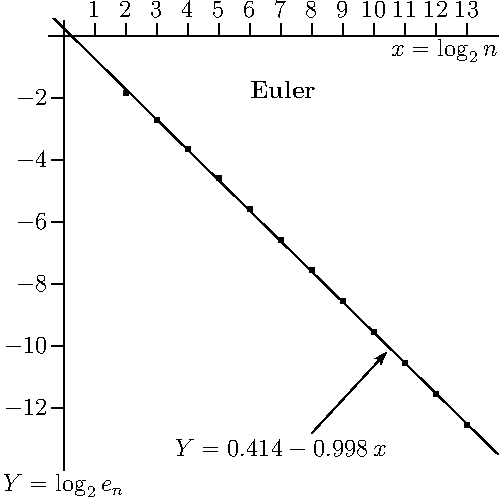
\includegraphics[scale=0.95]{euler_error.pdf}
%    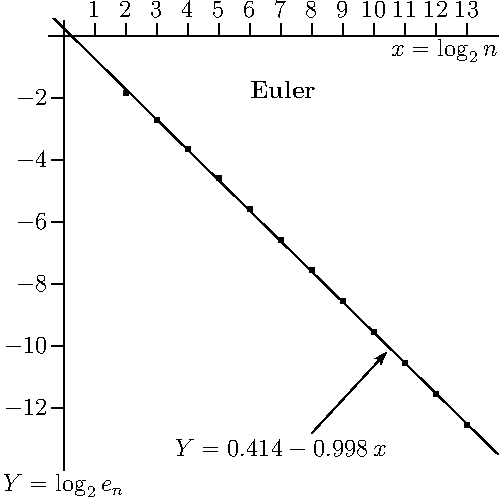
\includegraphics{euler_error.pdf}
\end{center}
\end{efig}

\begin{wfig}
\begin{center}
    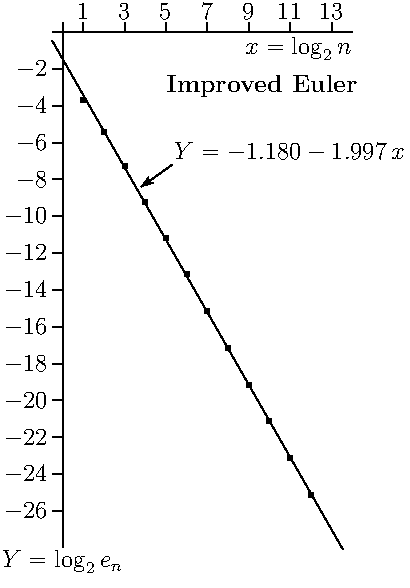
\includegraphics[scale=0.95]{imp_euler_error.pdf}\hskip0.5in
    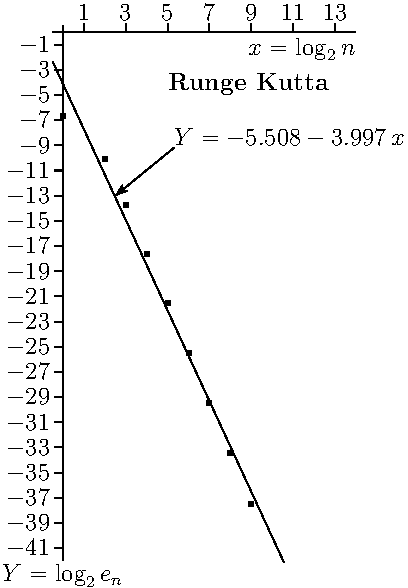
\includegraphics[scale=0.95]{runge_kutta_error.pdf}
\end{center}
\end{wfig}

\noindent
Each graph also contains a straight line, chosen by linear regression, to best fit the data. The method of linear regression for finding the straight line which best fits a given set of data points is covered in 
Example \eref{CLP3}{eg:MXMNlinReg} of the CLP-3 text.
The three straight lines have slopes $-0.998$ for Euler,
$-1.997$ for improved Euler and $-3.997$ for Runge Kutta. Reviewing (E1),
it sure looks like  $k=1$ for Euler, $k=2$ for 
improved Euler and $k=4$ for Runge-Kutta (at least if $k$ is integer).

So far we have only looked at the error in the approximate value of $y(t_f)$
as a function of the step size $h$ with $t_f$ held fixed. The graph below 
\vadjust{
\begin{wfig}
\begin{center}
    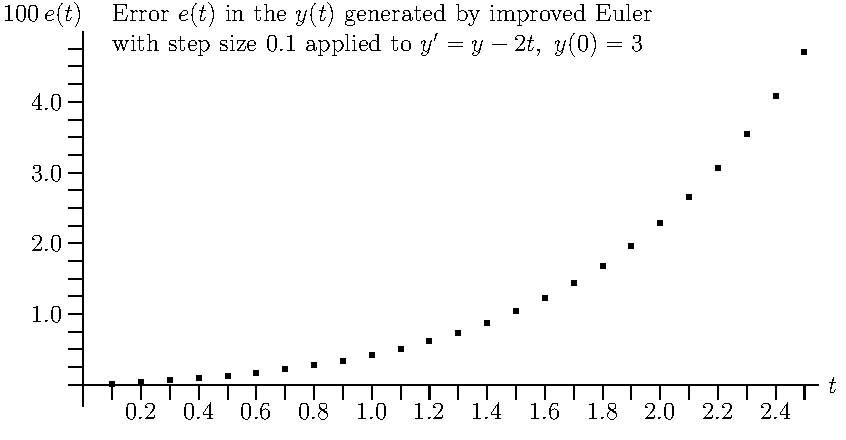
\includegraphics[scale=0.95]{t_error.pdf}
%    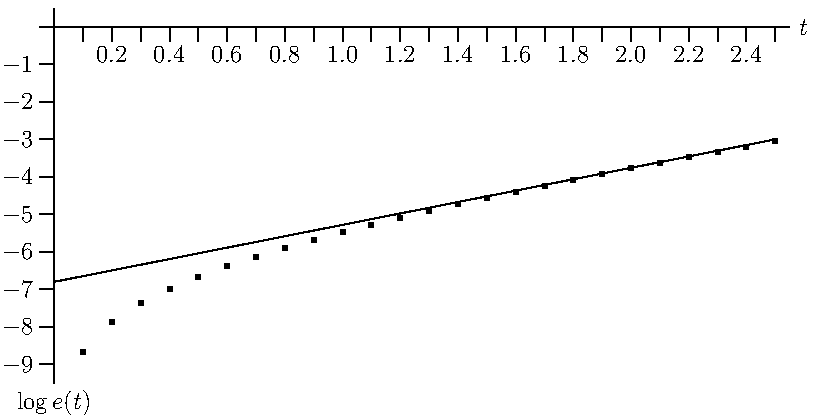
\includegraphics{t_log_error.pdf}
\end{center}
\end{wfig}
}
illustrates how the error behaves as a function of $t$, with $h$ held
fixed. That is, we hold the step size fixed and look at the error as a function of the distance, $t$, from the initial point. From the graph, it appears that the error grows exponentially with $t$. But it is not so easy to visually distinguish exponential curves from other upward 
curving curves. On the other hand, it is pretty easy to visually distinguish straight lines from other curves, and taking a logarithm converts 
the exponential curve $y=e^{kx}$ into  the straight line $Y=\log y = k\,x$.
Here is a graph of the logarithm, $\log e(t)$, of the error at time $t$, $e(t)$, against $t$. We have added a straight line as an aide to your eye.

\begin{wfig}
\begin{center}
    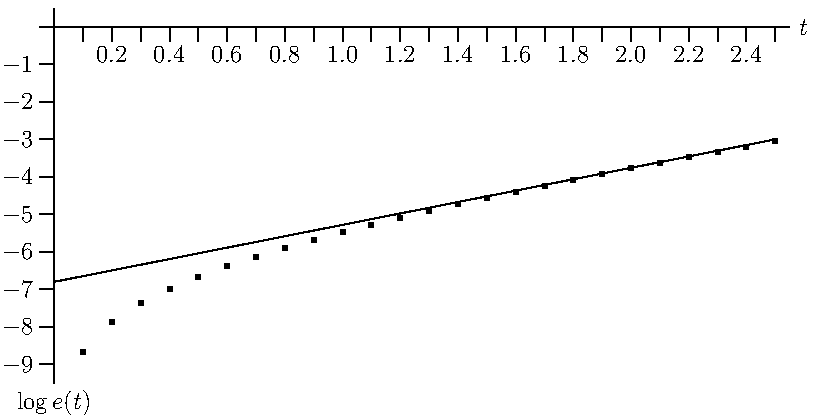
\includegraphics[scale=0.95]{t_log_error.pdf}
\end{center}
\end{wfig}

It looks like the $\log$ of the error grows very quickly initially, but then settles into a straight line. Hence it really does look like, at least in 
this example, except at the very beginning, the error $e(t)$ grows 
exponentially with $t$. 

The above numerical experiments have given a little intuition about the error behaviour of the Euler, improved Euler and Runge-Kutta methods. It's time to try and understand what is going on more rigorously.

%%%%%%%%%
\subsection{Local Truncation Error for Euler's Method}
%%%%%%%%%
We now try to develop some understanding as to why we got the above experimental
results. We start with the error generated by a single step of Euler's
method.

\begin{defn}[Local  truncation error]\label{def:locTrunc}
The (signed) error generated by a single step of Euler's method, under the assumptions 
that we start the step with the exact solution and that there is no roundoff 
error, is called the \emph{local truncation error} for Euler's method.
That is, if $\phi(t)$ obeys $\phi'(t) = f\big(t,\phi(t)\big)$ and
$\phi(t_n)=y_n$, and if $y_{n+1}=y_n+ hf(t_n,y_n)$,
then the local truncation error for Euler's method is
\begin{equation*}
\phi\big(t_{n+1}\big) -y_{n+1}
\end{equation*}
That is, it is difference between the exact value, $\phi\big(t_{n+1}\big)$,
and the approximate value generated by a single Euler method step, $y_{n+1}$, 
ignoring any numerical issues caused by storing numbers in a computer.
\end{defn}\noindent
Denote by $\phi(t)$ the exact solution to the initial value problem
\begin{equation*}
y'(t)=f(t,y)\qquad y(t_n)=y_n
\end{equation*}
That is, $\phi(t)$ obeys 
\begin{equation*}
\phi'(t) = f\big(t,\phi(t)\big)\qquad
\phi(t_n)=y_n
\end{equation*}
for all $t$. Now execute one more step of Euler's method with step size h:
\begin{equation*}
y_{n+1}=y_n+hf\big(t_n,y_n\big) 
\end{equation*}
Because we are assuming that $y_n=\phi(t_n)$
\begin{equation*}
y_{n+1}= \phi(t_n)+  hf\big(t_n,\phi(t_n)\big)
\end{equation*}
Because $\phi(t)$ is the exact solution, 
$\ \phi'(t_n) = f\big(t_n,\phi(t_n)\big)= f(t_n,y_n)\ $ and 
\begin{equation*}
y_{n+1}= \phi(t_n)+  h\phi'(t_n)
\end{equation*}
The local truncation error in $y_{n+1}$ is, by definition,  $\phi(t_{n+1})-y_{n+1}$. 

Taylor expanding (see (\eref{CLP1}{eq:taylorPoly}) 
in the CLP-1 text) $\phi(t_{n+1})=\phi(t_n+h)$  about $t_n$
\begin{equation*}
\phi(t_n+h)=\phi(t_n)+\phi'(t_n)h+\tfrac{1}{2} \phi''(t_n)h^2
                      +\tfrac{1}{3!}\phi'''(t_n)h^3+\cdots
\end{equation*}
so that
\begin{align*}
\phi(t_{n+1})-y_{n+1} 
&= \big[\phi(t_n)+\phi'(t_n)h+\tfrac{1}{2} \phi''(t_n)h^2
                     +\tfrac{1}{3!}\phi'''(t_n)h^3+\cdots\big]
-\big[\phi(t_n)+  h\phi'(t_n)\big]\notag\\
&= \tfrac{1}{2} \phi''(t_n)h^2+\tfrac{1}{3!}\phi'''(t_n)h^3+\cdots
\tag{E2}\end{align*}
Notice that the constant and $h^1$ terms have cancelled out. So the first term that appears is proportional to $h^2$. Since $h$ is typically a very small number, the $h^3$, $h^4$, $\cdots$ terms will usually be much smaller than 
the $h^2$ term.

We conclude that the local truncation error for Euler's method is $h^2$
times some unknown constant (we usually don't know the value of 
$\frac{1}{2} \phi''(t_n)$ because we don't usually know the solution 
$\phi(t)$ of the differential equation)
plus smaller terms that are proportional to $h^r$ with $r\ge 3$. 
This conclusion is typically written
\begin{impeqn}\label{eqn local trunc error Euler}
\begin{equation*}
\text{Local truncation error for Euler's method }= Kh^2+O(h^3)
\end{equation*}
\end{impeqn}
The symbol $O(h^3)$ is used to designate any function that, for small $h$,
is bounded by a constant times $h^3$. So, if $h$ is very small, $O(h^3)$ will be a lot smaller than $h^2$.

To get from an initial time $t=t_0$
to a final time $t=t_f$ using steps of size $h$ requires $(t_f-t_0)/h$ steps.
If each step were to introduce an error\footnote{For simplicity, we are assuming that $K$ takes the same value in every step. If, instead, there is a different $K$ in each of the $n=(t_f-t_0)/h$ steps, the final error would be $K_1h^2+K_2h^2+\cdots+K_nh^2+n O(h^3)= \bar K nh^2+n O(h^3)= \bar K(t_f-t_0)\, h+O(h^2)$, where $\bar K$ is the average of $K_1$, $K_2$, $\cdots$, $K_n$.} $Kh^2+O(h^3)$, then the final error in
the approximate value of $y(t_f)$ would be 
\begin{equation*}
\frac{t_f-t_0}{h}\ \Big[Kh^2+O(h^3)\Big]
           = K(t_f-t_0)\, h+O(h^2)
\end{equation*}
This very rough estimate is consistent with the experimental data for 
the dependence of error on step size with $t_f$ held fixed, shown on the 
first graph after Remark \ref{rmk:findk}. 
But it is not consistent with the experimental time dependence data above,
which shows the error growing exponentially, rather than linearly, in $t_f-t_0$.
 
We can get some rough understanding of this exponential growth as follows.
The general solution to $y'=y-2t$ is $y(t)=2+2t+c_0e^t$. The arbitrary constant,
$c_0$, is to be determined by initial conditions. When $y(0)=3$, $c_0=1$.
At the end of step 1, we have computed an approximation $y_1$ to $y(h)$.
This $y_1$ is not exactly $y(h)=2+2h+e^h$. Instead, it is a number that differs
from $2+2h+e^h$ by $O(h^2)$. We choose to write the number $y_1=2+2h+e^h+O(h^2)$ as $2+2h+(1+\epsilon)e^h$ with $\epsilon=e^{-h} O(h^2)$ 
of order of magnitude $h^2$. That is, we choose to write 
\begin{equation*}
y_1=2+2t+c_0e^t\Big|_{t=h}\qquad\text{with }c_0=1+\epsilon
\end{equation*}
If we were to make no further errors we would 
end up with the solution to
\begin{equation*}
y'=y-2t,\qquad y(h)= 2+2h+(1+\epsilon)e^h
\end{equation*}
which is\footnote{Note that this $y(t)$ obeys both the differential equation
$y'=y-2t$ and the initial condition $y(h)= 2+2h+(1+\epsilon)e^h$.}
\begin{align*}
y(t) &= 2+2t+(1+\epsilon)e^t
=2+2t+ e^t +\epsilon e^t \\
&=\phi(t) +\epsilon e^t
\end{align*}
So, once as error has been introduced, the natural time evolution of the
solutions to this differential equation cause the error to grow exponentially.
Other differential equations with other time evolution characteristics
will exhibit different $t_f$ dependence of errors\footnote{For example, if the solution is polynomial, then we might expect (by a similar argument) that the error also grows polynomially in $t_f$}. In the next
section, we show that, for many differential equations, errors grow at
worst exponentially with $t_f$. 

%%%%%%%%%%%%
\subsection{Global Truncation Error for Euler's Method}
%%%%%%%%%%%%%
Suppose once again that we are applying Euler's method with step size $h$ to
 the initial value problem 
\begin{align*}
y'(t)&=f(t,y) \\
y(0)&=y_0
\end{align*}
Denote by $\phi(t)$ the exact solution to the initial value problem and
by $y_n$ the approximation to $\phi(t_n),\ t_n=t_0+nh$, given by $n$ steps
of Euler's method (applied without roundoff error). 
\begin{defn}[Global  truncation error]\label{def:globalTrunc}
The (signed) error in $y_n$ is 
$\ 
\phi(t_n)-y_n
\ $ 
and is called the \emph{global truncation error} at time $t_n$. 
\end{defn}\noindent
The word ``truncation'' is supposed to signify that this error is due solely to
Euler's method and does not include any effects of roundoff error that might be introduced by our not writing down an infinite number of decimal digits for each number that we compute along the way.
We now derive a bound on the global truncation error. 

Define 
\begin{equation*}
\veps_n=\phi(t_n)-y_n
\end{equation*}
The first half of the derivation is to find a bound on $\veps_{n+1}$
in terms of $\veps_n$. 
\begin{equation*}
\begin{split}
\veps_{n+1}&=\phi(t_{n+1})-y_{n+1} \\
&=\phi(t_{n+1})-y_n-hf(t_n,y_n) \\
&=[\textcolor{red}{\phi(t_n)}-y_n]
  +h[\textcolor{blue}{f\big(t_n,\phi(t_n)\big)}-f(t_n,y_n)]
  +[\phi(t_{n+1})-\textcolor{red}{\phi(t_n)}
        -h\textcolor{blue}{f\big(t_n,\phi(t_n)\big)}]
\end{split}
\tag{E3}\end{equation*}
where we have massaged the expression into three manageable pieces.
\begin{itemize}
\item
The first $[\cdots]$ is exactly $\veps_n$. 
\item
The third $[\cdots]$ is exactly the local truncation error. Assuming that $|\phi''(t)|\le A$ for all $t$ of interest\footnote{We are assuming that the derivative $\phi'(t)$ doesn't change too rapidly. This will be the case if $f(t,y)$ is a reasonably smooth function.}, we can bound the third  $[\cdots]$ by
\begin{equation*}
\big|\phi(t_{n+1})-\phi(t_n)-hf\big(t_n,\phi(t_n)\big)\big|\le \half Ah^2
\end{equation*}
This bound follows quickly from the Taylor expansion with remainder 
((\eref{CLP1}{eq:taylorErrorQ}) in the CLP-1 text),
\begin{align*}
\phi(t_{n+1})&=\phi(t_n)+\phi'(t_n)h+\half \phi''(\tilde t)h^2 \\
&=\phi(t_n)+h\, f\big(t_n,\phi(t_n)\big)+\half \phi''(\tilde t)h^2
\end{align*}
for some $t_n<\tilde t<t_{n+1}$. 
\item
Finally, by the mean value theorem,
the magnitude of the second $[\cdots]$ is $h$ times
\begin{align*}
|f\big(t_n,\phi(t_n)\big)-f(t_n,y_n)|
&= F_{t_n}\big(\phi(t_n)\big)- F_{t_n}(y_n)
  &&\text{where}\quad F_{t_n}(y) = f\big(t_n,y\big) \\
&=\big|F'_{t_n}(\tilde y)\big| \,|\phi(t_n)-y_n|
   &&\text{for some $\tilde y$ between $y_n$ and $\phi(t_n)$} \\
&=\big|F'_{t_n}(\tilde y)\big| \,|\veps_n|\\
&\le B|\veps_n|
\end{align*}
assuming that $\big|F'_{t}(y)\big|\le B$ for all $t$ and $y$ of 
interest\footnote{Again, this will be the case if $f(t,y)$ is a reasonably smooth function.}. 
\end{itemize}
Substituting into (E3) gives
\begin{equation*}
|\veps_{n+1}|
\le |\veps_n| + Bh|\veps_n| +\half Ah^2
= (1+Bh)|\veps_n| +\half Ah^2
\tag{E4$_n$}
\end{equation*}
Hence the (bound on the) magnitude of the total error, $|\veps_{n+1}|$, consists of two parts. 
One part is the magnitude of the local truncation error, which is no more 
than $\half Ah^2$ and which is present even if we start the step with no 
error at all, i.e. with $\veps_n=0$.
The other part is due to the combined error from all previous steps.
This is the $\varepsilon_n$ term.
At the beginning of step number $n+1$, the combined error has magnitude
$|\veps_n|$. During the step, this error gets magnified by no more 
than a factor of $1+Bh$.

The second half of the derivation is to repeatedly apply (E4$_n$) with
$n=0,1,2,\cdots$. By definition $\phi(t_0)=y_0$ so that $\veps_0=0$, so
\begin{alignat*}{3}
&(\text{E4}_0)\implies|\veps_1|&&\le (1+Bh)|\veps_0| +\tfrac{A}{2}h^2
                        =\tfrac{A}{2} h^2 \\
&(\text{E4}_1)\implies|\veps_2|&&\le (1+Bh)|\veps_1| +\tfrac{A}{2} h^2
                               =(1+Bh)\tfrac{A}{2}h^2+\tfrac{A}{2}h^2 \\
&(\text{E4}_2)\implies|\veps_3|&&\le (1+Bh)|\veps_2| +\tfrac{A}{2}h^2
              =(1+Bh)^2\tfrac{A}{2}h^2+(1+Bh)\tfrac{A}{2}h^2+\tfrac{A}{2}h^2
\end{alignat*}
Continuing in this way 
\begin{equation*}
|\veps_n|\le 
       (1+Bh)^{n-1}\tfrac{A}{2}h^2+\cdots+(1+Bh)\tfrac{A}{2}h^2+\tfrac{A}{2}h^2
=\sum_{m=0}^{n-1} (1+Bh)^m \tfrac{A}{2}h^2
\end{equation*}
This is the beginning of a geometric series, and we can sum it up by using 
$\ \sum\limits_{m=0}^{n-1} ar^m=\frac{r^n-1}{r-1}a\ $ (which is Theorem
\ref{thm:INTspecialSums}(a))
with $\ a=\tfrac{A}{2}h^2\ $ and $\ r=1+Bh\ $ gives
\begin{equation*}
|\veps_n|\le \frac{(1+Bh)^n-1}{(1+Bh)-1}\frac{A}{2}h^2
=\frac{A}{2B}\big[(1+Bh)^n-1\big]h
\end{equation*}
We are interested in how this behaves as $t_n-t_0$ increases and/or $h$ decreases. Now $n=\frac{t_n-t_0}{h}$ so that $(1+Bh)^n=(1+Bh)^{(t_n-t_0)/h}$. When $h$ is small, the behaviour of $(1+Bh)^{(t_n-t_0)/h}$ is not so obvious. So we'll use a little trickery to make it easier to understand. Setting $x=Bh$ in 
\begin{equation*}
x\ge 0\implies 1+x\le 1+x+\frac{1}{2}x^2+\frac{1}{3!}x^3+\cdots = e^x
\end{equation*}
(the exponential series $e^x= 1+x+\frac{1}{2}x^2+\frac{1}{3!}x^3+\cdots$
was derived in Example~\ref{eg:expSeries})
gives\footnote{When $x=Bh$ is large, it is not wise to bound the linear $1+x$ by the much larger exponential $e^x$. However when $x$ is small, $1+x$ and $e^x$ are almost the same.} $1+Bh\le e^{Bh}$. Hence $(1+Bh)^n\le e^{Bhn}=e^{B(t_n-t_0)}$, 
since $t_n=t_0+nh$, and we arrive at the conclusion
\begin{impeqn}\label{glbl trunc error Euler}
\begin{equation*}
|\veps_n|\le \frac{A}{2B}\left[e^{B(t_n-t_0)}-1\right]h
\end{equation*}
\end{impeqn}
\noindent
which is of the form $K(t_f)h^k$ with $k=1$ and the coefficient $K(t_f)$ 
growing exponentially with $t_f-t_0$. If we keep $h$ fixed and increase $t_n$ we see exponential growth, but if we fix $t_n$ and decrease $h$ we see the error decrease linearly. 
This is just what our experimental data suggested.

\section{Variable Step Size Methods}

We now introduce a family of procedures that decide by themselves what step 
size to use. In all of these procedures the user specifies an acceptable error
rate and the procedure attempts to adjust the step size so that each step
introduces error at no more than that rate. That way the procedure uses a small step size when it is hard to get an accurate approximation, and a large step 
size when it is easy to get a good approximation.  

Suppose that we wish to generate an approximation to the initial value problem
\begin{equation*}
y'=f(t,y),\qquad
y(t_0)=y_0
\end{equation*}
for some range of $t$'s and we want the error introduced per
unit increase\footnote{We know that the error will get larger the
further we go in $t$. So it makes sense to try to limit the error per 
unit increase in $t$.} of $t$ to be no more than about some small fixed 
number $\veps$. This means that if $y_n\approx y(t_0+nh)$ and
$y_{n+1}\approx y(t+(n+1)h)$, then we want the local truncation error in the step from $y_n$ to $y_{n+1}$ to be no more than about $\veps h$. 
Suppose further that we have already produced the approximate solution as 
far as $t_n$. The rough strategy is as follows.
We do the step from $t_n$ to $t_n+h$ twice using two different 
algorithms, giving two different approximations to $y(t_{n+1})$, 
that we call $A_{1,n+1}$ and $A_{2,n+1}$. The two algorithms are chosen so that 
\begin{enumerate}[(1)]\itemsep1pt \parskip0pt \parsep0pt \itemindent0.25in
\item
we can use $A_{1,n+1}-A_{2,n+1}$ to compute an approximate local truncation 
error and
\item
for efficiency, the two algorithms use almost the same evaluations 
of $f$. Remember that evaluating the function $f$ is typically the most time-consuming part of our computation.
\end{enumerate}
In the event that the local truncation error, divided by $h$,
(i.e. the error per unit increase of $t$) is
smaller than $\veps$, we set $t_{n+1}=t_n+h$, accept $A_{2,n+1}$ 
as the approximate value\footnote{Better still, accept $A_{2,n+1}$ minus the computed approximate error in $A_{2,n+1}$ as the approximate value for $y(t_{n+1})$.} for $y(t_{n+1})$, and move on to the next step. Otherwise we 
pick, using what we have learned from $A_{1,n+1}-A_{2,n+1}$, a new trial 
step size $h$ and start over again at $t_n$.

Now for the details.
We start with a very simple minded procedure.

%%%%%%%%
\subsection{Euler and Euler-2step (preliminary version)}\label{ssec prelim E E2}
%%%%%%%%
Denote by $\phi(t)$ the exact solution to $y'=f(t,y)$ that satisfies the
initial condition $\phi(t_n)=y_n$. 
If we apply one step of Euler with step size $h$, giving
\begin{equation*}
A_{1,n+1}=y_n+hf(t_n,y_n)
\end{equation*}
we know, from \eqref{eqn local trunc error Euler}, that 
\begin{equation*}
A_{1,n+1}=\phi(t_n+h)+Kh^2+O(h^3)
\end{equation*}
The problem, of course, is that we don't know what the error is, even
approximately, because we don't know what the constant $K$ is. 
But we can estimate $K$ simply by redoing the step from $t_n$  to $t_n+h$
using a judiciously chosen second algorithm. There are a number of 
different second algorithms that will work. We call the simple algorithm 
that we use in this subsection Euler-2step\footnote{This name is begging for a 
dance related footnote and we invite the reader to supply their own.}. 
One step of Euler-2step with step size $h$ just consists of doing two steps 
of Euler with step size $h/2$:
\begin{equation*}
A_{2,n+1} = y_n+\tfrac{h}{2}f(t_n,y_n)
            +\tfrac{h}{2}f\big(t_n+\tfrac{h}{2},y_n+\tfrac{h}{2}f(t_n,y_n)\big)
\end{equation*}
Here, the first half-step took us from $y_n$ to 
$y_{\rm mid}=y_n+\frac{h}{2}f(t_n,y_n)$ and the second half-step took
us from $y_{\rm mid}$ to 
$y_{\rm mid}+\frac{h}{2}f\big(t_n+\frac{h}{2},y_{\rm mid}\big)$.
The local truncation error
introduced in the first half-step is $K(h/2)^2+O(h^3)$. That for
the second half-step is $K(h/2)^2+O(h^3)$ with the same\footnote{Because 
the two half-steps start at values of $t$ only $h/2$ apart, and we are 
thinking of $h$ as being very small, it should not be surprising that 
we can use the same value of $K$ in both. In case you don't believe us, 
we have included a derivation of the local truncation error for Euler-2step 
later in this appendix.} $K$, though with a different $O(h^3)$.
All together
\begin{align*}
A_{2,n+1}&=\phi(t_n+h)+\big[ K\big(\tfrac{h}{2}\big)^2+O(h^3)\big]
                   + \big[K\big(\tfrac{h}{2}\big)^2+O(h^3)\big] \\
&=\phi(t_n+h)+\half Kh^2+O(h^3)
\end{align*}
The difference is\footnote{Recall that every time the symbol $O(h^3)$ is 
used it can stand for a different function that is bounded by some 
constant times $h^3$ for small $h$. Thus $O(h^3)-O(h^3)$ need not be zero, 
but is $O(h^3)$. What is important here, is that if $K$ is not zero and if $h$ is very small, then $O(h^3)$ is much smaller than $\half Kh^2$.}
\begin{align*}
A_{1,n+1}-A_{2,n+1}&=\big[\phi(t_n+h)+Kh^2+O(h^3)\big]
             -\big[\phi(t_n+h)-\half Kh^2-O(h^3)\big] \\
&=\half Kh^2+O(h^3)
\end{align*}
So if we do one step of both Euler and Euler-2step, we can estimate
\begin{equation*}
\half Kh^2=A_{1,n+1}-A_{2,n+1}+O(h^3)
\end{equation*}
We now know that in the step just completed Euler-2step introduced an error 
of about  $\half Kh^2\approx A_{1,n+1}-A_{2,n+1}$. 
That is, the current error rate is about
$r=\frac{|A_{1,n+1}-A_{2,n+1}|}{h}\approx\half |K| h$ per unit increase of $t$.
\begin{itemize}
\item  
If this $r=\frac{|A_{1,n+1}-A_{2,n+1}|}{h}>\veps$, we reject\footnote{The measured error rate, $r$,  is bigger than the desired error rate $\veps$. That means that it is harder to get the accuracy we want than we thought. So we have to take smaller steps.} $A_{2,n+1}$ 
and repeat the current step with a new trial step size chosen so that 
$\half |K|(\text{new }h)<\veps$, i.e. $\frac{r}{h}(\text{new }h)<\veps$. 
To give ourselves a small safety margin, we could use\footnote{We don't want to make the new $h$ too close to $\frac{\veps}{r}{h}$ since we are only estimating things and we might end up with an error rate bigger that $\veps$. On the other hand, we don't want to make the new $h$ too small because that means too
much work --- so we choose it to be just a little smaller than $\frac{\veps}{r}{h}$ $\ldots$ say $0.9\frac{\veps}{r}{h}$ .} 
\begin{equation*}
\text{new }h=0.9\,\frac{\veps}{r}\,h
\end{equation*}
\item
If $r=\frac{|A_{1,n+1}-A_{2,n+1}|}{h}<\veps$ we can accept\footnote{The measured error rate, $r$,  is smaller than the desired error rate $\veps$. That means that it is easier to get the accuracy we want than we thought. So we can make the next step larger.} 
$A_{2,n+1}$ as an approximate  value for $y(t_{n+1})$, with $t_{n+1}=t_n+h$, 
and move on to the next step, starting with the new trial step size\footnote{Note that in this case $\frac{\veps}{r}>1$. So the new $h$ can be bigger than the last $h$.} 
\begin{equation*}
\text{new } h=0.9\,\frac{\veps}{r}\,h
\end{equation*}
\end{itemize}
That is our preliminary version of the Euler/Euler-2step variable step size method. We call it the preliminary version, because we will shortly tweak it 
to get a much more efficient procedure.

\begin{eg}\label{prelim E E2}
As a concrete example, suppose that our problem is 
\begin{equation*}
y(0)=e^{-2},\ y'=8(1-2t)y,\ \veps=0.1
\end{equation*}
and that we have gotten as far as
\begin{equation*}
t_n=0.33,\ y_n=0.75,\ \ \text{trial }h=0.094
\end{equation*}
Then, using $E=|A_{1,n+1}-A_{2,n+1}|$ to denote the magnitude of the 
estimated local truncation error in $A_{2,n+1}$ and $r$ the corresponding 
error rate
\begin{align*}
f(t_n,y_n)&=8(1-2\times 0.33) 0.75=2.04 \\
A_{1,n+1}&=y_n+hf(t_n,y_n)=0.75+0.094\times 2.04=0.942 \\[0.1in]
y_{\rm mid}&=y_n+\tfrac{h}{2}f(t_n,y_n)
                   =0.75+\tfrac{0.094}{2}\times 2.04=0.846 \\
f\big(t_n+\tfrac{h}{2},y_{\rm mid}\big)
&=8\Big[1-2\big(0.33+\tfrac{0.094}{2}\big)\Big]0.846=1.66 \\
A_{2,n+1}&=y_{\rm mid}+\tfrac{h}{2}f(t_n+\tfrac{h}{2},y_{\rm mid})
          =0.846+\tfrac{0.094}{2}1.66=0.924\\[0.1in]
E&=|A_{1,n+1}-A_{2,n+1}|=|0.942-0.924|=0.018\\
r&=\frac{|E|}{h}=\frac{0.018}{0.094}=0.19
\end{align*}
Since $r=0.19>\veps=0.1\,$, the current step size  
is unacceptable and we have to recompute with the new step size
\begin{equation*}
\text{new } h=0.9\frac{\veps}{r}(\text{old }h)
            =0.9\ \frac{0.1}{0.19}\ 0.094
            =0.045
\end{equation*}
to give
\begin{align*}
f(t_n,y_n)&=8(1-2\times0.33)0.75=2.04 \\
A_{1,n+1}&=y_n+hf(t_n,y_n)=0.75+0.045\times 2.04=0.842 \\[0.1in]
y_{\rm mid}&=y_n+\tfrac{h}{2}f(t_n,y_n)
                 =0.75+\tfrac{0.045}{2}\times 2.04=0.796 \\
f\big(t_n+\tfrac{h}{2},y_{\rm mid}\big)
&=8\Big[1-2\big(0.33+\tfrac{0.045}{2}\big)\Big]0.796=1.88 \\
A_{2,n+1}&=y_{\text{mid}}
               +\tfrac{h}{2}f(t_n +\tfrac{h}{2},y_{\rm mid})
          =0.796+\tfrac{0.045}{2}1.88
          =0.838 \\[0.1in]
E&=A_{1.n+1}-A_{2.n+1}=0.842-0.838=0.004 \\
r&=\frac{|E|}{h}=\frac{0.004}{0.045}=0.09
\end{align*}
This time $\,r=0.09<\veps=0.1\,$, is acceptable
so we set $t_{n+1}=0.33+0.045=0.375$ and 
\begin{equation*}
y_{n+1}=A_{2,n+1}=0.838
\end{equation*}
The initial trial step size from $t_{n+1}$ to $t_{n+2}$ is
\begin{equation*}
\text{new }h = 0.9\frac{\veps}{r}(\text{old }h)
  =0.9\,\frac{0.1}{0.09}\,.045=.045
\end{equation*}
By a fluke, it has turned out that the new $h$ is the same as the old $h$ (to three decimal places). If $r$ had been significantly smaller than $\veps$, then the new $h$ would have been signficantly bigger than the old $h$ - indicating that it is (relatively) easy to estimate things in this region, making a larger step size sufficient.
\end{eg}

As we said above, we will shortly upgrade the above variable step size method,
that we are calling the preliminary version of the Euler/Euler-2step method,  
to get a much more efficient procedure. Before we do so, let's pause 
to investigate a little how well our preliminary procedure does at 
controlling the rate of error production.
 
We have been referring, loosely, to $\veps$ as the desired rate for introduction
of error, by our variable step size method, as $t$ advances. 
If the rate of increase of error were exactly $\veps$, then at final time
$t_f$ the accumulated error would be exactly $\veps(t_f-t_0)$. But our 
algorithm actually chooses the step size $h$ for each step so that the 
estimated local truncation error in $A_{2,n+1}$ for that step is about 
$\veps h$. We have seen that, once some local truncation error has been 
introduced, its contribution to the global truncation error can 
grow exponentially with $t_f$.

Here are the results of a numerical experiment that illustrate this effect. 
In this experiment, the above preliminary Euler/Euler-2step method is applied to the initial value problem
$\ 
y'=t-2y,\ 
y(0)=3
\ $
for $\veps=\frac{1}{16},\frac{1}{32},\cdots$ (ten different values)
and for $t_f=0.2,\ 0.4,\ \cdots,\ 3.8$.
Here  is a plot of the resulting
$\frac{{\rm actual\ error\ at\ }t=t_f}{\veps t_f}$ against $t_f$.
\vadjust{
\begin{efig}
\begin{center}
    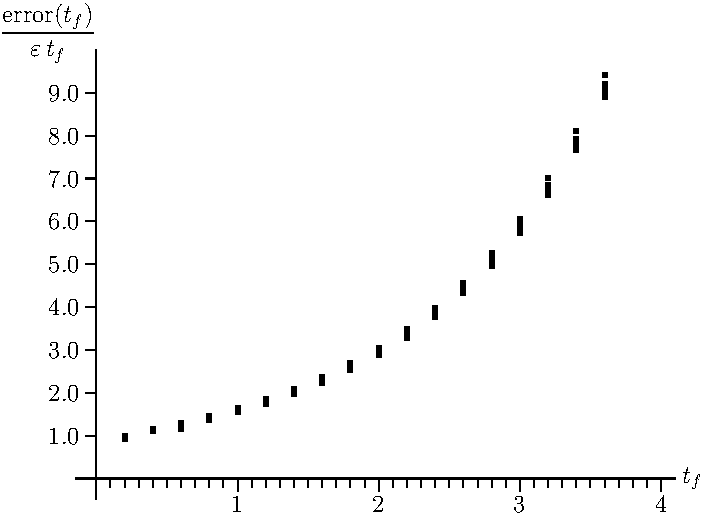
\includegraphics[scale=0.9]{vble_error.pdf}
%    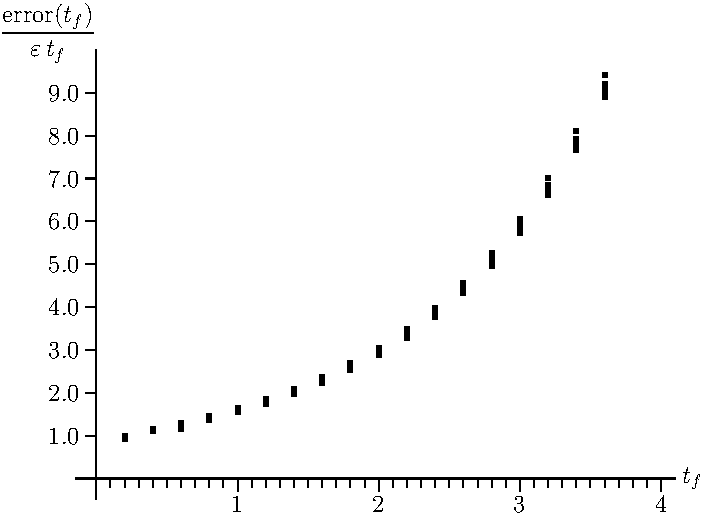
\includegraphics{vble_error.pdf}
\end{center}
\end{efig}
}
If the rate of introduction of error were exactly $\veps$, we would have
$\frac{{\rm actual\ error\ at\ }t=t_f}{\veps t_f}=1$.
There is a small square on the graph for each different pair $\veps,t_f$. So for
each value of $t_f$ there are ten (possibly overlapping) squares on the line $x=t_f$. This numerical
experiment suggests that $\frac{{\rm actual\ error\ at\ }t=t_f}{\veps t_f}$
is relatively independent of $\veps$ and starts, when $t_f$ is small, 
at about one, as we want, but grows (perhaps exponentially) with $t_f$.

%%%%%%%%
\subsection{Euler and Euler-2step (final version)}\label{ssec final E E2}
%%%%%%%%

We are now ready to use a sneaky bit of arithemtic to supercharge our Euler/Euler-2step method.
As in our development of the preliminary version of the method,
denote by $\phi(t)$ the exact solution to $y'=f(t,y)$ that satisfies the
initial condition $\phi(t_n)=y_n$. We have seen, at the beginning of 
\S\ref{ssec prelim E E2}, that
applying one step of Euler with step size $h$, gives
\begin{align}
A_{1,n+1}&=y_n+hf(t_n,y_n) \notag\\
         &=\phi(t_n+h)+Kh^2+O(h^3)
\tag{E5}\end{align}
and applying one step of Euler-2step with step size $h$ (i.e. applying two 
steps of Euler with step size $h/2$) gives
\begin{align}
A_{2,n+1} &= y_n+\tfrac{h}{2}f(t_n,y_n)
 +\tfrac{h}{2}f\big(t_n+\tfrac{h}{2}\,,\,y_n+\tfrac{h}{2}f(t_n,y_n)\big)\notag\\
          &=\phi(t_n+h)+\tfrac{1}{2} Kh^2+O(h^3)
\tag{E6}\end{align}
because the local truncation error introduced in the first half-step was $K(h/2)^2+O(h^3)$ and that introduced in the second half-step was 
$K(h/2)^2+O(h^3)$.
Now here is the sneaky bit. Equations (E5) and (E6) are very similar and we can eliminate all $Kh^2$'s by subtracting (E5) from $2$ times (E6). This gives
\begin{equation*}
\text{2(E6)$-$(E5):}\qquad
2A_{2,n+1}-A_{1,n+1} = \phi(t_n+h) +O(h^3)
\end{equation*}
(no more $h^2$ term!) or
\begin{equation*}
\phi(t_n+h)= 2A_{2,n+1}-A_{1,n+1}+O(h^3)
\tag{E7}\end{equation*} 
which tells us that choosing
\begin{equation*}
y_{n+1}=2A_{2,n+1}-A_{1,n+1}
\tag{E8}\end{equation*}
would give a local truncation error of order $h^3$, rather than 
the order $h^2$ of the preliminary Euler/Euler-2step method.
To convert the preliminary version of the Euler/Euler-2step algorithm 
to the final version, we just replace $y_{n+1}=A_{2,n+1}$ by
$y_{n+1} = 2A_{2,n+1}-A_{1,n+1}$:

\begin{impeqn}[Euler/Euler-2step Method]\label{full E E2}
Given $\veps>0$, $t_n$, $y_n$ and the current step size $h$
\begin{itemize}
\item compute
\begin{align*}
A_{1,n+1}&=y_n+hf(t_n,y_n) \\
A_{2,n+1} &= y_n+\tfrac{h}{2}f(t_n,y_n)
    +\tfrac{h}{2}f\big(t_n+\tfrac{h}{2}\,,\,y_n+\tfrac{h}{2}f(t_n,y_n)\big)\\
r&=\frac{|A_{1,n+1}-A_{2,n+1}|}{h}
\end{align*}

\item
If $r>\veps$, repeat the first bullet but with the new step size
\begin{equation*}
(\text{new }h)=0.9\,\frac{\veps}{r}\,(\text{old }h)
\end{equation*}

\item
If $r<\veps$ set
\begin{align*}
t_{n+1}&=t_n+h \\
y_{n+1}&=2A_{2,n+1}-A_{1,n+1}\quad\text{and the new trial step size} \\
(\text{new } h)&=0.9\,\frac{\veps}{r}\,(\text{old }h)
\end{align*}
and move on to the next step. 
\end{itemize}
\end{impeqn}\noindent
Note that when $r<\veps$, we have $\frac{r}{\veps}h> h$ which indicates that the new $h$ can be larger than the old $h$. We include the $0.9$ to be careful not to make the error of the next step too big.

Let's think a bit about how our final Euler/Euler-2step method should perform.
\begin{itemize}
\item
The step size here, as in the preliminary version, is chosen so that
the local truncation error in $A_{2,n+1}$ per unit increase of $t$,
namely $r=\frac{|A_{1,n+1}-A_{2,n+1}|}{h}\approx\frac{Kh^2/2}{h}=\frac{K}{2}h$, 
is approximately $\veps$. So $h$ is roughly proportional to $\veps$. 
\item
On the other hand, (E7) shows that, in the full method, local truncation 
error is being added to $y_{n+1}$ at a rate of $\frac{O(h^3)}{h}=O(h^2)$ 
per unit increase in $t$. 
\item
So one would expect that local truncation increases the error at a rate proportional to $\veps^2$ per unit increase in $t$. 
\item
If the rate of increase of error were exactly a constant time $\veps^2$, 
then the error accumulated between the initial time $t=0$ and the final 
time $t=t_f$ would be exactly a constant times $\veps^2\,t_f$. 
\item
However we have seen that, once some local truncation error has been introduced, its contribution to the global error can grow exponentially with $t_f$. So we would expect that, under the full Euler/Euler-2step method, 
$\frac{{\rm actual\ error\ at\ }t=t_f}{\veps^2 t_f}$ to be more or less independent of $\veps$, but still growing exponentially in $t_f$.
\end{itemize}
Here are the results of a numerical experiment that illustrate this. 
In this experiment, the above final Euler/Euler-2step method, 
\eqref{full E E2}, is applied to the initial value problem
$\ 
y'=t-2y,\ 
y(0)=3
\ $
for $\veps=\frac{1}{16},\frac{1}{32},\cdots$ (ten different values)
and for $t_f=0.2,\ 0.4,\ \cdots,\ 3.8$. In the following plot, there is a small 
square for the resulting $\frac{{\rm actual\ error\ at\ }t=t_f}{\veps^2 t_f}$ 
for each different pair $\veps,t_f$.


\begin{efig}
\begin{center}
%    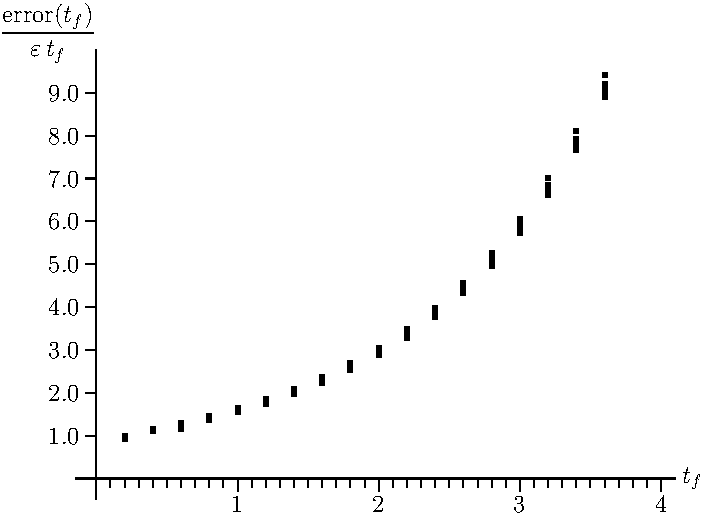
\includegraphics[scale=1.3]{vble_error.pdf}
    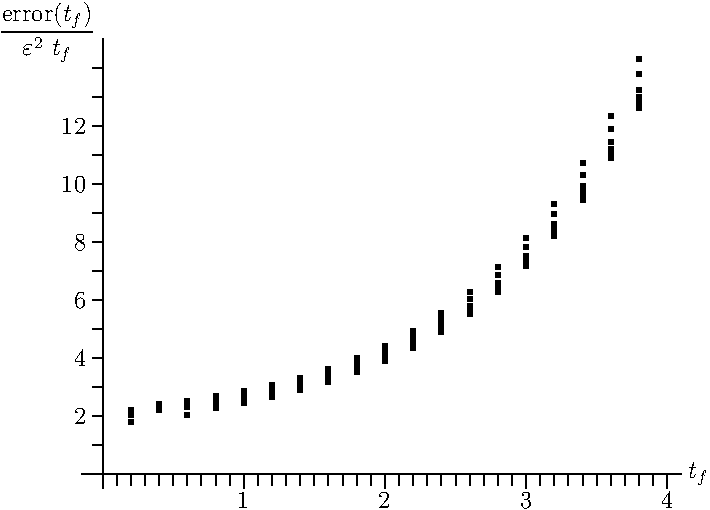
\includegraphics{vble4_error.pdf}
\end{center}
\end{efig}
It does indeed look like $\frac{{\rm actual\ error\ at\ }t=t_f}{\veps^2 t_f}$
is relatively independent of $\veps$ but grows (perhaps exponentially) with $t_f$. Note that $\frac{{\rm actual\ error\ at\ }t=t_f}{\veps^2 t_f}$ contains a factor of $\veps^2$ in the denominator. The actual error rate 
$\frac{{\rm actual\ error\ at\ }t=t_f}{t_f}$ is much smaller than is suggested by the graph.

%%%%%%%%%%%%%
\subsection{Fehlberg's Method}
%%%%%%%%%%%%%

Of course, in practice more efficient and more accurate methods\footnote{There are a very large number of such methods. We will only look briefly at a couple of the simpler ones. The interested reader can find more by search engining for such keywords as ``Runge-Kutta methods'' and ``adaptive step size''. } than 
Euler and Euler-2step are used. Fehlberg's method\footnote{E. Fehlberg, 
NASA Technical Report R315 (1969) and NASA Technical Report R287 (1968).} 
uses improved Euler and a second more accurate method. Each step involves 
three calculations of $f$:
\begin{align*}
f_{1,n}&=f(t_n,y_n) \\
f_{2,n}&=f(t_n+h,y_n+hf_{1,n}) \\
f_{3,n}&=f\left(t_n+\tfrac{h}{2},y_n+\tfrac{h}{4}[f_{1,n}+f_{2,n}]\right)
\end{align*}
Once these three evaluations have been made, the method generates two
approximations for $y(t_n+h)$:
\begin{align*}
A_{1,n+1}&=y_n+\tfrac{h}{2}\left[f_{1,n}+f_{2,n}\right] \\
A_{2,n+1}&=y_n+\tfrac{h}{6}\left[f_{1,n}+f_{2,n}+4f_{3,n}\right]
\end{align*}
Denote by $\phi(t)$ the exact solution to $y'=f(t,y)$ that satisfies 
the initial condition $\phi(t_n)=y_n$.  Now $A_{1,n+1}$ is just the $y_{n+1}$
produced by the improved Euler's method. The local truncation error for the
improved Euler's method is of order $h^3$, one power of $h$ smaller than that
for Euler's method. So
\begin{equation*}
A_{1,n+1} = \phi(t_n+h) + Kh^3+O(h^4) 
\end{equation*}
and it turns out\footnote{The interested reader can find Fehlberg's original paper online (at NASA!) and follow the derivation. It requires careful Taylor expansions and then clever algebra to cancel the bigger error terms.} that
\begin{equation*}
A_{2,n+1} = \phi(t_n+h) + O(h^4) 
\end{equation*}
So the  error in $A_{1,n+1}$ is
\begin{align*}
E&=\big|Kh^3+O(h^4)\big|
  =\big|A_{1,n+1}-\phi(t_n+h)\big|+O(h^4) \\
  &=\big|A_{1,n+1}-A_{2,n+1}\big|+O(h^4)
\end{align*}
and our estimate for rate at which error is being introduced into $A_{1,n+1}$ is
\begin{equation*}
r=\frac{|A_{1,n+1}-A_{2,n+1}|}{h}\approx |K|h^2
\end{equation*}
per unit increase of $t$.
\begin{itemize}
\item
If $r>\veps$ we redo this step with a new trial step size chosen so that 
$|K|(\text{new }h)^2<\veps$, i.e. $\frac{r}{h^2}(\text{new }h)^2<\veps$. 
With our traditional safety factor, we take
\begin{equation*}
\text{new }h=0.9\sqrt{\frac{\veps}{r}}\,h\qquad
\text{(the new $h$ is smaller)}
\end{equation*}
\item
If $r\le \veps$ we set $t_{n+1}=t_n+h$ and $y_{n+1}=A_{2,n+1}$ (since 
$A_{2,n+1}$ should be considerably more accurate than $A_{1,n+1}$) 
and move on to the next step with trial step size 
\begin{equation*}
\text{new }h=0.9\sqrt{\frac{\veps}{r}}\,h\qquad
\text{(the new $h$ is usually bigger)}
\end{equation*}
\end{itemize}
%%%%%%%%%%%%%%%%%%%%%%%%%%%%%%%%%%%
\subsection{The Kutta-Merson Process}
%%%%%%%%%%%%%%%%%%%%%%%%%%%%%%%%%%%

The Kutta-Merson process\footnote{
R.H. Merson, ``An operational method for the study of integration processes'' , Proc. Symp. Data Processing , Weapons Res. Establ. Salisbury , Salisbury (1957) pp. 110--125.
%A reference is L. Fox, Numerical Solution of Ordinary and Partial Differential Equations.
} uses two variations of 
the Runge-Kutta method. Each step involves five calculations\footnote{Like the other methods described above, the coefficients $1/3$, $1/6$, $1/8$ etc.
are chosen so as to cancel larger error terms. While determining the
correct choice of coefficients is not conceptually difficult, it does take some
work and is beyond the scope of this appendix. The interested reader should
search-engine their way to a discussion of adaptive Runge-Kutta methods.} 
of $f$:
\begin{align*}
k_{1,n}&=f(t_n,y_n) \\
k_{2,n}&=f\big(t_n+\tfrac{1}{3}h,y_n+\tfrac{1}{3}hk_{1,n}\big)\\
k_{3,n}&=
  f\big(t_n+\tfrac{1}{3}h,y_n+\tfrac{1}{6}hk_{1,n}+\tfrac{1}{6}hk_{2,n}\big) \\
k_{4,n}&=
   f\big(t_n+\tfrac{1}{2}h,y_n+\tfrac{1}{8}hk_{1,n}+\tfrac{3}{8}hk_{3,n}\big) \\
k_{5,n}&=
   f\big(t_n+h,y_n+\tfrac{1}{2}hk_{1,n}-\tfrac{3}{2}hk_{3,n}+2hk_{4,n}\big)
\end{align*}
Once these five evaluations have been made, the process generates two
approximations for $y(t_n+h)$:
\begin{align*}
A_{1,n+1}&=y_n+h\left[\tfrac{1}{2}k_{1,n}-\tfrac{3}{2}k_{3,n}+2k_{4,n}\right] \\
A_{2,n+1}&=y_n+h\left[\tfrac{1}{6}k_{1,n}+\tfrac{2}{3}k_{4,n}
                   +\tfrac{1}{6}k_{5,n}\right]
\end{align*}
The (signed) error in $A_{1,n+1}$ is $\frac{1}{120}h^5K+O(h^6)$ while that in
$A_{2,n+1}$ is $\frac{1}{720}h^5K+O(h^6)$ with the same constant $K$. 
So $A_{1,n+1}-A_{2,n+1} = \frac{5}{720}Kh^5+O(h^6)$ and the unknown
constant $K$ can be determined, to within an error $O(h)$, by
\begin{equation*}
K=\frac{720}{5\,h^5}(A_{1,n+1}-A_{2,n+1})
\end{equation*}
and the approximate (signed) error in $A_{2,n+1}$ and its corresponding rate 
per unit increase of $t$ are
\begin{align*}
E&=\frac{1}{720}K h^5=\frac{1}{5}(A_{1,n+1}-A_{2,n+1}) \\
r=\frac{|E|}{h}&=\frac{1}{720}|K| h^4=\frac{1}{5\,h}\big|A_{1,n+1}-A_{2,n+1}\big|
\end{align*}
\begin{itemize}
\item
If $r>\veps$ we redo this step with a new trial step size chosen so that
$\frac{1}{720}|K|(\text{new h})^4<\veps$, 
i.e. $\frac{r}{h^4}(\text{new }h)^4<\veps$. 
With our traditional safety factor, we take
\begin{equation*}
\text{new }h=0.9\left(\frac{\veps}{r}\right)^{1/4}\,h
\end{equation*}
\item
If $r\le \veps$ we set $t_{n+1}=t_n+h$ and $y_{n+1}=A_{2,n+1}-E$ (since $E$ is
our estimate of the signed error in $A_{2,n+1}$) and move on to the next step with trial step size 
\begin{equation*}
\text{new }h=0.9\left(\frac{\veps}{r}\right)^{1/4}\,h
\end{equation*}
\end{itemize}

%%%%%%%%%%%%%%%%%%%%%%%%%%%%%%%%%%%%%%%%%%
\subsection{The Local Truncation Error for Euler-2step}
%%%%%%%%%%%%%%%%%%%%%%%%%%%%%%%%%%%%%%%%%%

In our description of Euler/Euler-2step above we simply stated the local truncation error without an explanation. In this section, we show how it may be derived. We note that very similar calculations underpin the other methods we have described. 

In this section, we will be using partial derivatives and, in particular, the chain rule for functions of two variables. That material is covered in Chapter 2 of the CLP-3 text. If you are not yet comfortable with it, you can either take our word for those bits, or you can delay reading this section until you have learned a little multivariable calculus.  

Recall that, by definition, the local truncation error for an algorithm
is the (signed) error generated by a single step of the algorithm, under the 
assumptions that we start the step with the exact solution and that there
is no roundoff error\footnote{We should note that in serious big
numerical computations, one really does have to take rounding errors into account because they can cause serious problems. The interested reader should search-engine their way to the story of Edward Lorenz's numerical simulations and the beginnings of chaos theory. Unfortunately we simply do not have space in this text to discuss all aspects of mathematics.}
Denote by $\phi(t)$ the exact solution to 
\begin{align*}
y'(t)&=f(t,y) \\
y(t_n)&=y_n
\end{align*}
In other words, $\phi(t)$ obeys 
\begin{align*}
\phi'(t) &= f\big(t,\phi(t)\big)\qquad\text{ for all }t \\
\phi(t_n)&=y_n
\end{align*}
In particular $\phi'(t_n)=f\big(t_n,\phi(t_n)\big)=f(t_n,y_n)$ and,
carefully using the chain rule, which is (\eref{CLP3}{eqn chain rule A}) in the CLP-3 text, 
\begin{align*}
\phi''(t_n)&=\diff{}{t}f\big(t,\phi(t)\big)\Big|_{t=t_n}
 =\Big[f_t\big(t,\phi(t)\big)+f_y\big(t,\phi(t)\big)\phi'(t)\Big]_{t=t_n} \\
&=f_t(t_n,y_n)+f_y(t_n,y_n)\,f(t_n,y_n)
\tag{E9}\end{align*}
Remember that $f_t$ is the partial derivative of $f$ with respect to $t$, 
and that $f_y$ is the partial derivative of $f$ with respect to $y$. We'll need (E9) below.

By definition, the local truncation error for Euler is
\begin{equation*}
E_1(h)=\phi(t_n+h)-y_n-hf\big(t_n,y_n\big) 
\end{equation*}
while that for Euler-2step is
\begin{equation*}
E_2(h)=\phi(t_n+h)-y_n-\tfrac{h}{2}f(t_n,y_n)
-\tfrac{h}{2}f\big(t_n+\tfrac{h}{2},y_n+\tfrac{h}{2}f(t_n,y_n)\big)
\end{equation*}
To understand how $E_1(h)$ and $E_2(h)$ behave for small $h$ we can use Taylor expansions ((\eref{CLP1}{eq:taylorPoly}) in the CLP-1 text) to write them as power series in $h$. To be precise, we use
\begin{equation*}
g(h)=g(0)+g'(0)\,h+\half g''(0)\,h^2+O(h^3)
\end{equation*}
to expand both $E_1(h)$ and $E_2(h)$ in powers of $h$ to order $h^2$.
Note that, in the expression for $E_1(h)$,  $t_n$ and $y_n$ are constants ---
they do not vary with $h$. So computing derivatives of $E_1(h)$ with
respect to $h$ is actually quite simple.
\begin{alignat*}{5}
E_1(h)&=\phi(t_n+h)-y_n-hf\big(t_n,y_n\big)\qquad &
             E_1(0)&=\phi(t_n)-y_n=0 \\
E'_1(h)&=\phi'(t_n+h)-f\big(t_n,y_n\big) &
         E'_1(0)&=\phi'(t_n)-f\big(t_n,y_n\big)=0 \\
E''_1(h)&=\phi''(t_n+h) &
         E''_1(0)&=\phi''(t_n) 
\end{alignat*}
By Taylor, the local truncation error for Euler obeys
\begin{impeqn}\label{Euler 1step}
\begin{equation*}
E_1(h)=\half\phi''(t_n)h^2+O(h^3)=Kh^2+O(h^3)\qquad\text{with }
                      K=\half\phi''(t_n)
\end{equation*}
\end{impeqn}
Computing arguments of $E_2(h)$ with respect to $h$ is a little harder, since $h$ now appears in the arguments of the function $f$. As a consequence, we have to include some partial derivatives.
\begin{align*}
E_2(h)&=\phi(t_n+h)-y_n-\frac{h}{2}f(t_n,y_n)
     -\frac{h}{2}f\Big(t_n+\frac{h}{2},y_n+\frac{h}{2}f(t_n,y_n)\Big) 
\\[0.1in]
E'_2(h)&=\phi'(t_n+h)-\frac{1}{2}f(t_n,y_n)
-\frac{1}{2}f\Big(t_n+\frac{h}{2},y_n+\frac{h}{2}f(t_n,y_n)\Big) \\
&\hskip2.5in-\frac{h}{2}
\underbrace{\diff{}{h} f\Big(t_n+\frac{h}{2},y_n+\frac{h}{2}f(t_n,y_n)
     \Big)}_{\text{leave this expression as is for now}}  
\\[0.1in]
E''_2(h)&=\phi''(t_n+h)
-2\times\frac{1}{2}
\underbrace{\diff{}{h} f\Big(t_n+\frac{h}{2},y_n+\frac{h}{2}f(t_n,y_n)
      \Big)}_{\text{leave this one too}} \\
&\hskip2.5in-\frac{h}{2}
\underbrace{\difftwo{}{h}f\Big(t_n+\frac{h}{2},y_n+\frac{h}{2}f(t_n,y_n)
      \Big)}_{\text{and leave this one too}}
\end{align*}
Since we only need $E_2(h)$ and its derivatives at $h=0$, we don't have to compute the $\difftwo{f}{h}$ term (thankfully) and we also do not need to
compute the $\diff{f}{h}$ term in $E_2'$. We do, however, need  
$\diff{f}{h}\Big|_{h=0}$ for $E_2''(0)$.
\begin{align*}
E_2(0)&=\phi(t_n)-y_n=0 \\[0.1in]
E'_2(0)&=\phi'(t_n)-\frac{1}{2}f(t_n,y_n)-\frac{1}{2}f(t_n,y_n)=0 \\[0.1in]
E''_2(0)&=\phi''(t_n)-\diff{}{h}
f\Big(t_n+\frac{h}{2},y_n+\frac{h}{2}f(t_n,y_n)\Big)\Big|_{h=0} \\
&=\phi''(t_n)-
\frac{1}{2} f_t\Big(t_n+\frac{h}{2},y_n+\frac{h}{2}f(t_n,y_n)\Big)\Big|_{h=0} \\
&\hskip1.5in -\frac{1}{2} f(t_n,y_n)\, f_y\Big(t_n+\frac{h}{2},y_n+\frac{h}{2}f(t_n,y_n)\Big)\Big|_{h=0} \\
&=\phi''(t_n)- \frac{1}{2}f_t(t_n,y_n)-\frac{1}{2}f_y(t_n,y_n)\, f(t_n,y_n) \\
&=\half\phi''(t_n)\qquad\text{by (E9)}
\end{align*}
By Taylor, the local truncation error for Euler-2step obeys
\begin{impeqn}\label{Euler 2step}
\begin{equation*}
E_2(h)=\frac{1}{4}\phi''(t_n)\,h^2+O(h^3)
=\half Kh^2+O(h^3)\qquad{\rm with\ }K=\half\phi''(t_n)
\end{equation*}
\end{impeqn}\noindent
Observe that the $K$ in (\ref{Euler 2step}) is identical to the $K$ in 
(\ref{Euler 1step}). This is exactly what we needed in our analysis of 
Sections \ref{ssec prelim E E2} and \ref{ssec final E E2}.







